I% Chapter Template

\chapter{Vector Structure and Operations} % Main chapter title

\label{VectorStructure} % Change X to a consecutive number; for referencing this chapter elsewhere, use \ref{ChapterX}

\lhead{Vector Structure. \emph{Vector Structure}} % Change X to a consecutive number; this is for the header on each page - perhaps a shortened title

%----------------------------------------------------------------------------------------
%	SECTION - Radix Balanced Vectors
%----------------------------------------------------------------------------------------

\section{Radix Balanced Vectors}

%-----------------------------------
%	SUBSECTION - Tree structure
%-----------------------------------

\subsection{Tree structure}
% describe tree: balancing, filling, block sizes
% why structure helps with operations implementation 
% hint why radix?  


\begin{figure}[h!]
  \centering
  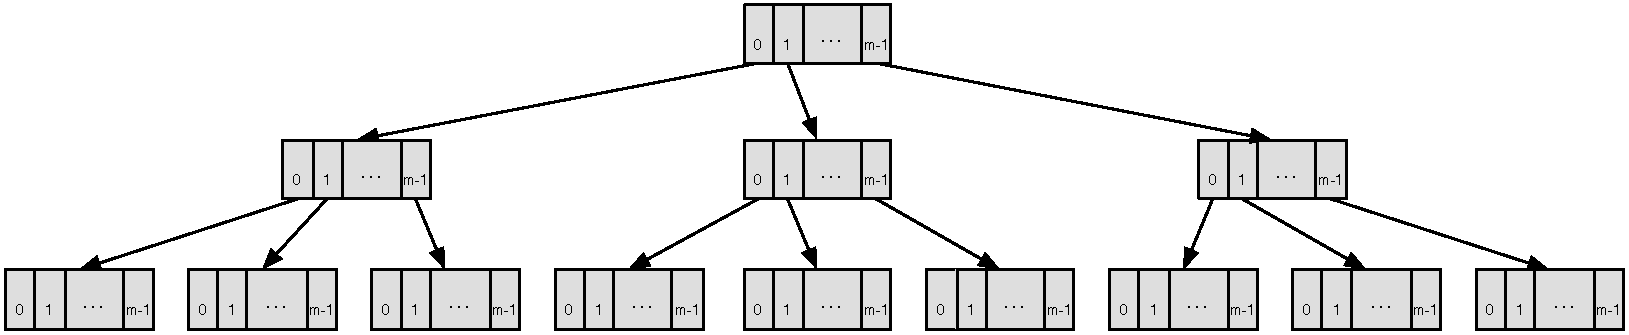
\includegraphics[width=\textwidth]{Figures/Radix_Balanced}
  \label{badix_balanced}
  \caption{Radix Balanced Tree Structure}
\end{figure}



%-----------------------------------
%	SUBSECTION - Operations
%-----------------------------------
\subsection{Operations}
% List core operations
% naive implementation just as high level guide
% Hint of displays and transient states


%-----------------------------------
%	SUBSUBSECTION - Apply
%-----------------------------------

\subsubsection{Apply}
% used in head and last
% performance log_32(n), hint of displays

\begin{lstlisting}[frame=single]
def apply(index: Int): A = {
  def getElem(node: Array[AnyRef], depth: Int): A = {
    val indexInNode = // get subindex
    if(depth == 1) node(indexInNode)
    else getElem(node(indexInNode), depth-1) 
  }
  getElem(vectorRoot, vectorDepth)
}
\end{lstlisting}

%-----------------------------------
%	SUBSUBSECTION - Updated
%-----------------------------------

\subsubsection{Updated}
% base implementation needs to update the whole branch
% with transient states, local updates can be amortised

\begin{lstlisting}[frame=single]
def updated(index: Int, elem: A) = {
  def updatedNode(node: Array[AnyRef], depth: Int) = {
    val indexInNode = // compute index
    val copy = clone(node)
    if(depth == 1) {
      copy(indexInNode) = elem
    } else {
      copy(indexInNode) = 
        updatedNode(node(indexInNode), depth-1)
    }
    copy
  }
  new Vector(updatedNode(vectorRoot, vectorDepth), ...)
}
\end{lstlisting}

%-----------------------------------
%	SUBSUBSECTION - Additions
%-----------------------------------

\subsubsection{Additions}

\paragraph{Append}
% base implementation needs to update the whole branch
% performance log_32(n), hint of transient to amortise consecutive appends are amortised

\paragraph{Prepend}
% base implementation needs to update the whole branch
% shift top and start index
% performance log_32(n), hint of transient to amortise consecutive appends are amortised

\paragraph{Concatenation and Insert}
% describe high level implementation in vector
%% describe branch rebalancing 
% performance O(n)


%-----------------------------------
%	SUBSUBSECTION - Splits
%-----------------------------------

\subsubsection{Splits}
% used in tail, init, take, takeRight, drop, dropRight
% describe implementation in vector
% performance log_32(n) 


%----------------------------------------------------------------------------------------
%	SECTION - Parallel Vectors
%----------------------------------------------------------------------------------------

\section{Parallel Vectors}
% why are  parallel vector useful
% how are they paralellized (wraps an vector)
% why do they suffer performance wise (no efficient concat)
% fork-join pool

%-----------------------------------
%	SUBSUBSECTION - Splitter
%-----------------------------------

\subsection{Splitter (Iterator)}
% split into half 
To divide the work into tasks for thread pool, a splitter is used to iterate over all elements of the collection. Splitters are a special kind of iterator that can be split at any time into some partition of the remaining elements. In the case of sequences the splitter should retain the original order. The most common implementation consists in dividing the remaining elements into two half. 

The current implementation of the immutable parallel  vector \cite{scalaParVector211}  uses the common division into 2 parts for it splitter. The drop and take operations are used divide the vector for the two new splitters.

%-----------------------------------
%	SUBSUBSECTION - Combiner
%-----------------------------------

\subsection{Combiner (Builder)}
% lazy combiner
Combiners are used to merge the results from different tasks (in methods like map, filter, collect, ...) into the new collection. Combiners are a special kind of builder that is able to merge to partial results efficiently. When it's impossible to implement efficient combination operation, usually a lazy combiner is used. The lazy combiner is one keeps all the it's sub-combiners in an array buffer and only when the end result is needed they are combined. This is a fairly efficient implementation but does not take full advantage of parallelism. 

The current implementation of the immutable parallel vector \cite{scalaParVector211} use the lazy approach because of it's inefficient concatenation operation. One of the consequences of this is that the parallel operations will always be bounded by this sequential combination of elements, which can be beaten by the sequential version in many cases.
 

%----------------------------------------------------------------------------------------
%	SECTION - Relaxed Radix Balanced Vectors
%----------------------------------------------------------------------------------------

\section{Relaxed Radix Balanced Vectors}

%-----------------------------------
%	SUBSECTION - Tree structure
%-----------------------------------

\subsection{Relaxed Tree structure}
% describe tree: balancing, filling, block sizes
% describe sizes array and where it is kept (change from left to right for indexing simplification)
% mention size of nodes and null sizes
% unbalanced trees can only be generated by concatenation, and splits

\begin{figure}[h!]
  \centering
  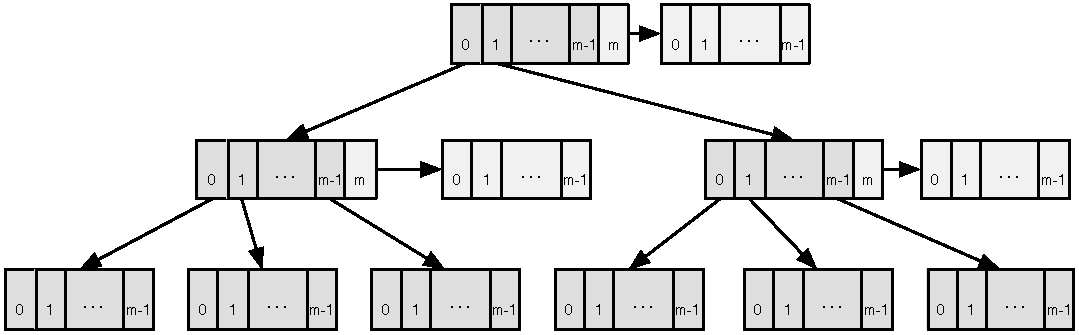
\includegraphics[width=\textwidth]{Figures/Relaxed_Radix_balanced}
  \label{Relaxed_Radix_balanced}
  \caption{Radix Balanced Tree}
\end{figure}

\begin{figure}[h!]
  \centering
  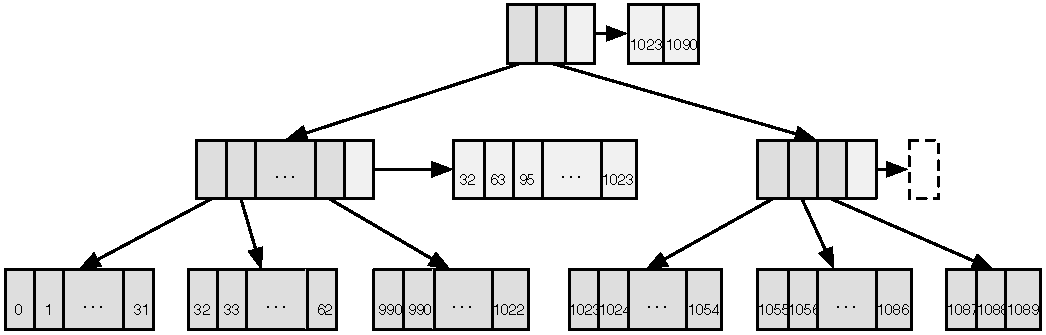
\includegraphics[width=\textwidth]{Figures/Relaxed_radix_example}
  \label{Relaxed_radix_example}
  \caption{Relaxed radix example}
\end{figure}

%-----------------------------------
%	SUBSECTION - Operations
%-----------------------------------
\subsection{Relaxed Operations}
% describe how the implementation uses relaxed radix when necessary and uses radix based operation when possible

%-----------------------------------
%	SUBSUBSECTION - Apply
%-----------------------------------

\subsubsection{Apply (get element at index)}
% describe the way to get the node indices in an unbalanced node


%-----------------------------------
%	SUBSUBSECTION - Updated
%-----------------------------------

\subsubsection{Updated}
% doesn't change much, the sizes do not need to be updated, they jus need to be copied. Going to the correct position still may needs to access the sizes.

%-----------------------------------
%	SUBSUBSECTION - Additions
%-----------------------------------

\subsubsection{Additions}

%-----------------------------------
\paragraph{Append}
% difference is that the the sizes may need to be updated
% performance log_32(n), remind hint of transient to amortise consecutive appends are amortised

\paragraph{Prepend}
% describe different implementation
% hint the 


%-----------------------------------
\paragraph{Concatenation}
% describe high level implementation in rrbvector
%% describe branch rebalancing 
% performance log_32(n)

\begin{figure}[h!]
  \centering
  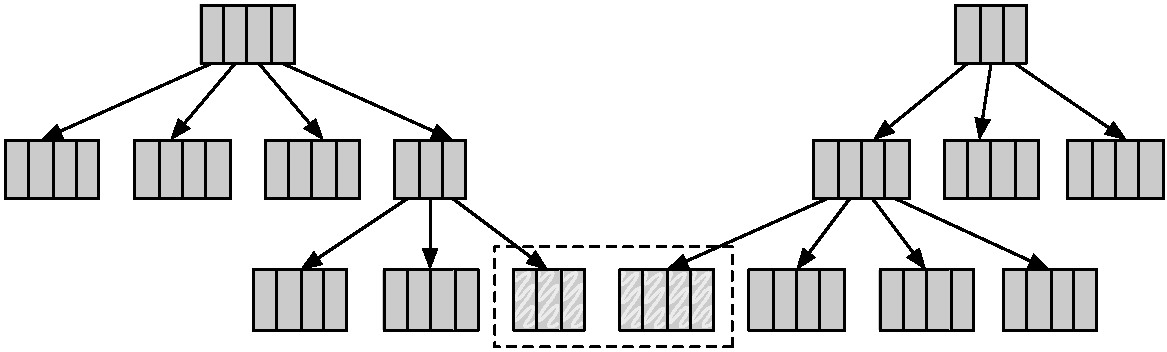
\includegraphics[width=\textwidth]{Figures/Concat0.pdf}
  \label{Concat0Benchmarks}
  \caption{Concatenation example with blocks of size 4: Rebalancing level 0}
\end{figure}

\begin{figure}[h!]
  \centering
  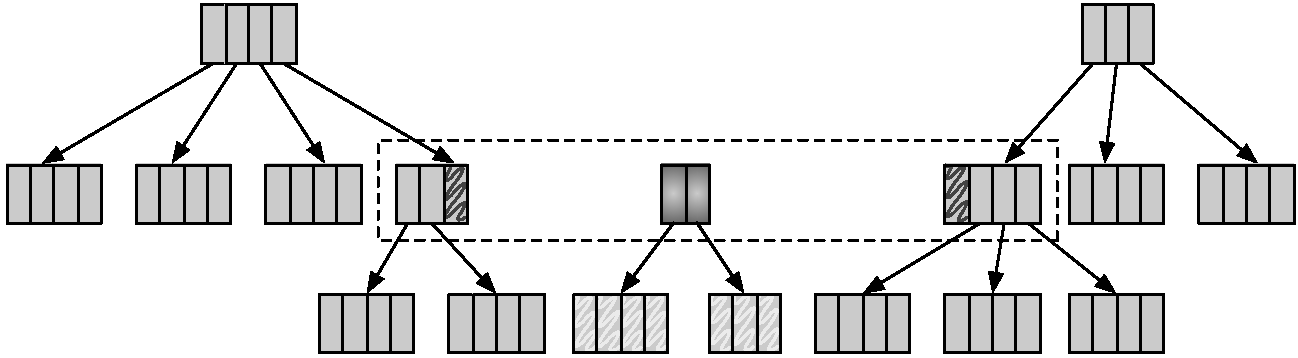
\includegraphics[width=\textwidth]{Figures/Concat1.pdf}
  \label{Concat1Benchmarks}
  \caption{Concatenation example with blocks of size 4: Rebalancing level 1}
\end{figure}

\begin{figure}[h!]
  \centering
  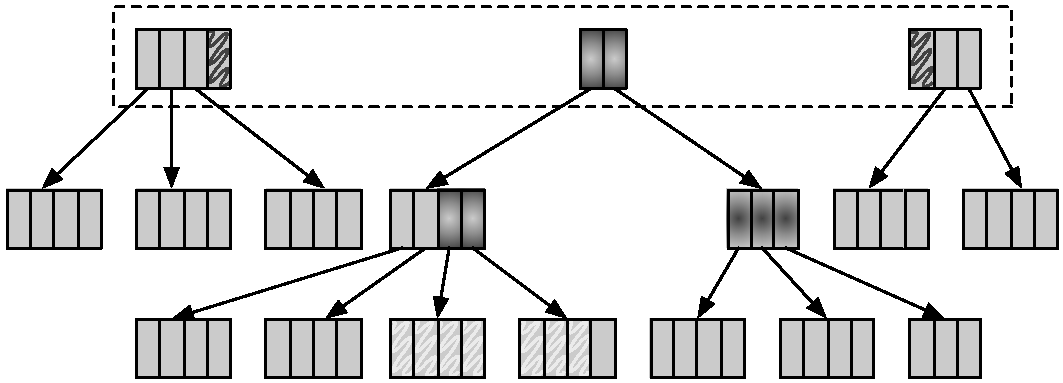
\includegraphics[width=\textwidth]{Figures/Concat2.pdf}
  \label{Concat2Benchmarks}
  \caption{Concatenation example with blocks of size 4: Rebalancing level 2}
\end{figure}

\begin{figure}[h!]
  \centering
  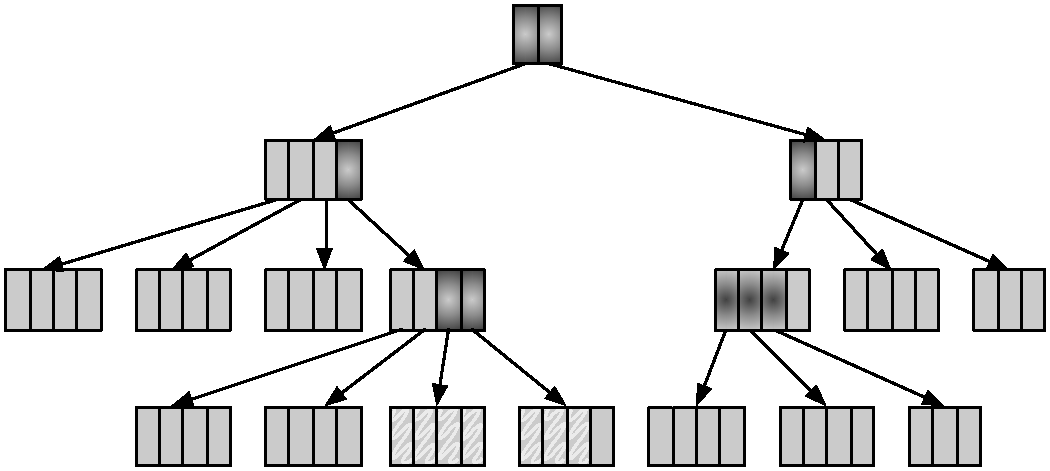
\includegraphics[width=\textwidth]{Figures/Concat3.pdf}
  \label{Concat3Benchmarks}
  \caption{Concatenation example with blocks of size 4: Rebalancing level 3}
\end{figure}


%-----------------------------------
\paragraph{Insert}
% new operation
% describe simple implementation using split and concat 
% performance log_32 (from split + concat)
% hint at possible optimization by inserting directly and using transient states (take advantage of locality)



%-----------------------------------
%	SUBSUBSECTION - Splits
%-----------------------------------

\subsubsection{Splits}
% used in tail, init, take, takeRight, drop, dropRight
% describe difference between the implementation (null and shift vs. cut and update size)

%-----------------------------------
%	SUBSUBSECTION - Splits
%-----------------------------------

\subsubsection{Parallel Vector}
% Combine: trivial expansion from builder
%% heuristic: try to construct balanced trees 
% Split into subtrees two, take the nearest power of 32 to the half


